\documentclass[11pt, a4paper]{article}

% ── Packages ──────────────────────────────────────────────────────────────────
\usepackage[a4paper, top=2.5cm, bottom=2.5cm, left=2.8cm, right=2.8cm]{geometry}
\usepackage[T1]{fontenc}
\usepackage[utf8]{inputenc}
\usepackage[spanish]{babel}
\usepackage{lmodern}
\usepackage{microtype}
\usepackage{graphicx}
\usepackage{subcaption}
\usepackage{booktabs}
\usepackage{array}
\usepackage{multirow}
\usepackage{xcolor}
\usepackage{amsmath}
\usepackage{hyperref}
\usepackage{parskip}
\usepackage{titlesec}
\usepackage{fancyhdr}
\usepackage{float}

\graphicspath{{../outputs/figures/}}

% ── Colors ────────────────────────────────────────────────────────────────────
\definecolor{accent}{RGB}{41, 98, 155}
\definecolor{lightgray}{RGB}{245, 245, 245}
\definecolor{darkgray}{RGB}{80, 80, 80}

% ── Hyperref ──────────────────────────────────────────────────────────────────
\hypersetup{
    colorlinks = true,
    linkcolor  = accent,
    urlcolor   = accent,
    citecolor  = accent,
}

% ── Section formatting ────────────────────────────────────────────────────────
\titleformat{\section}{\large\bfseries\color{accent}}{{\thesection.}}{0.5em}{}[\vspace{-4pt}\rule{\linewidth}{0.4pt}]
\titleformat{\subsection}{\normalsize\bfseries\color{darkgray}}{\thesubsection.}{0.5em}{}

% ── Header / Footer ───────────────────────────────────────────────────────────
\pagestyle{fancy}
\fancyhf{}
\fancyhead[L]{\small\textcolor{darkgray}{Clasificación de imágenes CCTV - Puertos Inteligentes}}
\fancyhead[R]{\small\textcolor{darkgray}{AIDA - Práctica 1}}
\fancyfoot[C]{\small\thepage}
\renewcommand{\headrulewidth}{0.3pt}

% ── Columna para tablas ───────────────────────────────────────────────────────
\newcolumntype{C}[1]{>{\centering\arraybackslash}p{#1}}

% ══════════════════════════════════════════════════════════════════════════════
\begin{document}

% ── Title ─────────────────────────────────────────────────────────────────────
\begin{titlepage}
    \centering
    \vspace*{2cm}
    {\Large\bfseries Clasificación de Imágenes CCTV\\[0.4em]
    en Entornos Portuarios\par}
    \vspace{0.5cm}
    \rule{10cm}{0.5pt}
    \vspace{0.5cm}

    {\large Detección de barcos y estado de atraque mediante redes convolucionales\par}
    \vspace{2cm}

    {\normalsize
    \textbf{Autor:} Nicolás Aller Ponte\\[0.3em]
    \textbf{Asignatura:} Análisis e Interpretación de Datos Audiovisuales (AIDA)\\[0.3em]
    \textbf{Práctica:} P1 - Clasificación con CNNs\\[0.3em]
    \textbf{Dataset:} Smartports CCTV Port Surveillance\\[0.3em]
    }
    \vspace{1.5cm}

    \begin{abstract}
    \noindent
    Este trabajo aborda dos tareas de clasificación binaria sobre imágenes de
    cámaras CCTV de un puerto: (1)~detección de barco (\textit{Ship/No-Ship}) y
    (2)~estado de atraque (\textit{Docked/Undocked}). Se comparan tres
    arquitecturas - una CNN ligera entrenada desde cero (\textsc{SimpleCNN}),
    una variante inspirada en ConvNeXt (\textsc{MiniConvNeXt}) y
    \textsc{ResNet18} con \textit{fine-tuning} desde ImageNet - bajo un esquema
    de validación cruzada de 5 iteraciones. Adicionalmente se
    evalúa una estrategia de \textit{transfer learning} inter-tarea
    (Ship $\to$ Docked). \textsc{ResNet18} domina en ambas tareas, alcanzando
    AUC-ROC de 0.999 en Ship y 0.861 en Docked. El transfer learning
    inter-tarea no parece mejorar los resultados.
    \end{abstract}
\end{titlepage}

% ══════════════════════════════════════════════════════════════════════════════
\section{Introducción}

La automatización de la vigilancia portuaria es un caso de uso real y creciente
dentro de la visión por computador aplicada a entornos industriales. Disponer de
sistemas que detecten automáticamente la presencia de embarcaciones o su estado
de atraque reduce la dependencia de operadores humanos y permite integrar la
información en sistemas de gestión de tráfico marítimo.

En esta práctica se trabaja con el dataset \textit{Smartports CCTV}, brindado en la Asignatura, el cual contiene
imágenes de vigilancia capturadas en un puerto real. El problema se plantea como
dos tareas de clasificación binaria independientes:

\begin{itemize}
    \item \textbf{Ship/No-Ship}: ¿hay un barco visible en la imagen? (294 imágenes)
    \item \textbf{Docked/Undocked}: si hay barco, ¿está atracado? (184 imágenes)
\end{itemize}

El objetivo es comparar distintas estrategias de modelado, analizar el efecto
del \textit{data augmentation} y explorar si el conocimiento adquirido en la
primera tarea puede transferirse a la segunda.

% ══════════════════════════════════════════════════════════════════════════════
\section{Dataset}

\subsection{Descripción y distribución de clases}

El dataset consta de 294 imágenes JPEG en resolución variable, todas
redimensionadas a $224 \times 224$ píxeles antes de ser procesadas por los
modelos. Las etiquetas se distribuyen de la siguiente forma:

\begin{itemize}
    \item \textbf{Ship/No-Ship}: 184 imágenes con barco (62.6\%) y 110 sin barco
          (37.4\%). El desequilibrio leve se corrige aplicando
          \texttt{pos\_weight=0.598} en la función de pérdida
          \texttt{BCEWithLogitsLoss}.
    \item \textbf{Docked/Undocked}: 92 imágenes atracadas (50\%) y 92 no atracadas
          (50\%). Las clases están perfectamente balanceadas, por lo que no se
          aplica corrección de peso.
\end{itemize}

\subsection{Partición de datos}

Se emplea \textbf{validación cruzada estratificada de 5 iteraciones}
(\textit{5-Fold Stratified CV}). Dentro de cada fold, el conjunto de
entrenamiento se subdivide en un 75\%/25\% de entrenamiento efectivo y
validación, manteniendo la estratificación. Esto permite evaluar la variabilidad
del rendimiento entre particiones y obtener estimaciones estadísticamente robustas.

El tamaño reducido del dataset (294 y 184 imágenes) justifica esta decisión:
un \textit{hold-out} simple no aportaría suficiente fiabilidad estadística.

% ══════════════════════════════════════════════════════════════════════════════
\section{Arquitecturas y Metodología}

\subsection{Modelos comparados}

Se evalúan tres arquitecturas con niveles de complejidad y estrategias de
inicialización diferentes:

\begin{description}
    \item[\textsc{SimpleCNN}] Red convolucional ligera diseñada desde cero. Consta
    de tres bloques \texttt{Conv2D~$\to$~BN~$\to$~ReLU~$\to$~MaxPool} seguidos de
    un clasificador con \texttt{AdaptiveAvgPool} y una capa lineal de salida.
    Parámetros entrenables: $\sim$120k. Rápido pero limitada capacidad de aprendizaje.

    \item[\textsc{MiniConvNeXt}] Arquitectura inspirada en ConvNeXt,
    también entrenada desde cero. Emplea convoluciones \textit{depthwise} $7\times7$,
    \texttt{LayerNorm} y conexiones residuales en las capas (\textit{layer scale}).
    Etapas de dimensiones [40, 80, 160, 320] con profundidades [2, 2, 6, 2].
    Es más compleja que \textsc{SimpleCNN} pero requiere más datos para
    generalizar, puede no generar buenos resultados con un dataset como este y así será.

    \item[\textsc{ResNet18}] Arquitectura preentrenada en ImageNet
    (\texttt{IMAGENET1K\_V1}). La capa \texttt{fc} final se sustituye por una
    salida de dimensión~1 para clasificación binaria. Se entrena en dos fases:
    primero con el \textit{backbone} congelado (épocas 1--4), y a partir de la
    época~5 se descongela para \textit{fine-tuning} completo con
    $\text{lr} = 10^{-4}$.
\end{description}

\subsection{Configuración de entrenamiento}

\begin{center}
\begin{tabular}{ll}
\toprule
\textbf{Hiperparámetro} & \textbf{Valor} \\
\midrule
Optimizador         & Adam \\
LR (SimpleCNN / ConvNeXt) & $10^{-3}$ \\
LR (ResNet18)       & $10^{-4}$ \\
Scheduler           & ReduceLROnPlateau (factor 0.5, patience 3) \\
Función de pérdida  & BCEWithLogitsLoss \\
Batch size          & 16 \\
Épocas máximas      & 50 \\
Early stopping      & patience = 7 (sobre val\_loss) \\
\bottomrule
\end{tabular}
\end{center}

\subsection{Data augmentation}

Para evaluar su efecto se entrena cada configuración con y sin augmentation.
Las transformaciones aplicadas son: volteo horizontal aleatorio, rotación
($\pm15°$), variación de brillo/contraste y \textit{jitter} de color. La
normalización ImageNet se aplica en todos los casos.

% ══════════════════════════════════════════════════════════════════════════════
\section{Resultados: Ship / No-Ship}

\subsection{Rendimiento comparativo}

\begin{table}[H]
\centering
\caption{Resultados en test (media $\pm$ desv. típica, 5-Fold CV) - Ship/No-Ship.
         Métrica principal: AUC-ROC.}
\label{tab:ship}
\small
\begin{tabular}{llC{1.6cm}C{1.6cm}C{1.8cm}C{1.8cm}}
\toprule
\textbf{Modelo} & \textbf{Aug} & \textbf{Acc} & \textbf{F1} & \textbf{AUC-ROC} & \textbf{AUC-PR} \\
\midrule
\multirow{2}{*}{ResNet18}   & No  & 0.980 ± 0.013 & 0.984 ± 0.010 & \textbf{0.999 ± 0.001} & 0.999 ± 0.001 \\
                             & Sí  & 0.973 ± 0.023 & 0.979 ± 0.017 & \textbf{0.999 ± 0.001} & 0.999 ± 0.001 \\
\midrule
\multirow{2}{*}{SimpleCNN}  & No  & 0.846 ± 0.020 & 0.882 ± 0.016 & 0.891 ± 0.024 & 0.918 ± 0.032 \\
                             & Sí  & 0.772 ± 0.058 & 0.826 ± 0.032 & 0.814 ± 0.039 & 0.862 ± 0.047 \\
\midrule
\multirow{2}{*}{MiniConvNeXt} & No & 0.779 ± 0.092 & 0.827 ± 0.062 & 0.836 ± 0.088 & 0.898 ± 0.059 \\
                               & Sí & 0.697 ± 0.078 & 0.754 ± 0.072 & 0.765 ± 0.052 & 0.837 ± 0.025 \\
\bottomrule
\end{tabular}
\end{table}

\subsection{Análisis}

La tarea de detección de barcos resulta \textbf{relativamente sencilla para
ResNet18}, que alcanza un AUC-ROC prácticamente perfecto (0.999) gracias a los
features de bajo nivel aprendidos en ImageNet. La diferencia con los modelos
entrenados desde cero es notable: \textsc{SimpleCNN} logra un AUC-ROC de 0.891,
razonable para una red tan ligera, mientras que \textsc{MiniConvNeXt} sorprende
con resultados inferiores a pesar de ser más compleja, como indicamos antes su complejidad complica su capacidad
de entrenamiento en un dataset de estas caracteristicas ($\sim$230 imágenes de entrenamiento efectivas).

\begin{figure}[H]
    \centering
    \begin{subfigure}[t]{0.48\textwidth}
        \centering
        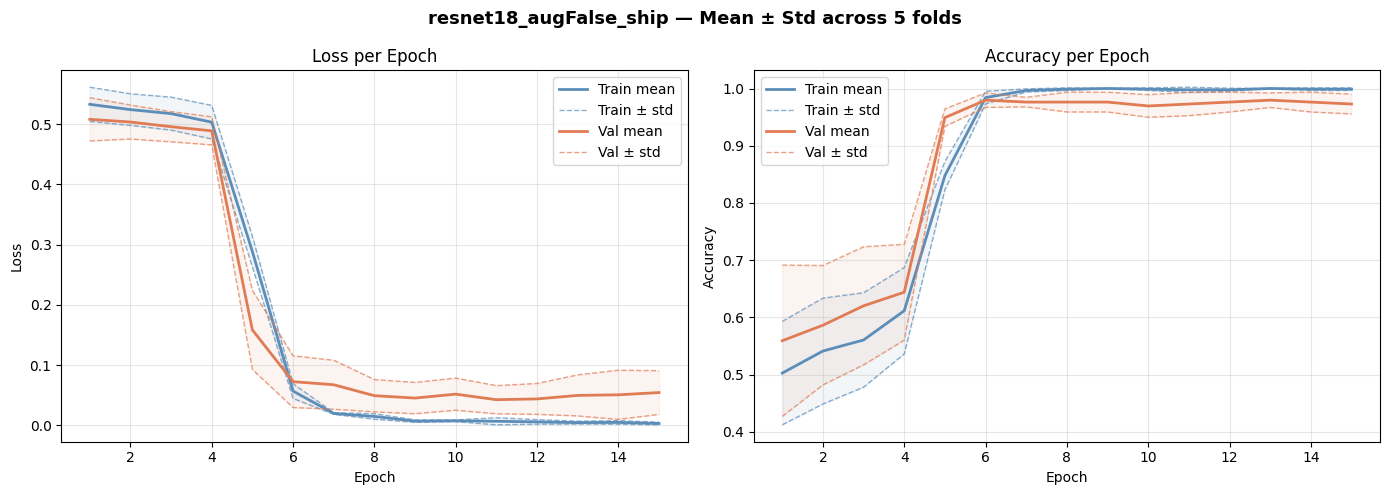
\includegraphics[width=\linewidth]{resnet18_augFalse_ship_mean_std_history.png}
        \caption{Historial de entrenamiento - ResNet18 (sin aug, ship).
                 El descongelado del \textit{backbone} en época 5 produce
                 una caída pronunciada de la pérdida de validación.}
    \end{subfigure}
    \hfill
    \begin{subfigure}[t]{0.48\textwidth}
        \centering
        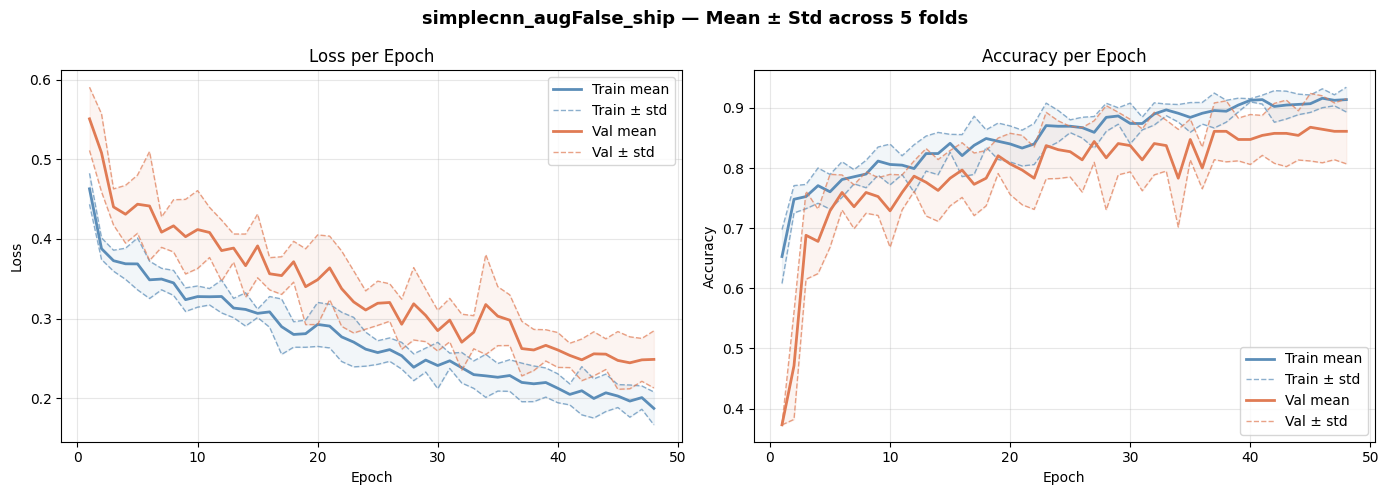
\includegraphics[width=\linewidth]{simplecnn_augFalse_ship_mean_std_history.png}
        \caption{Historial de entrenamiento - SimpleCNN (sin aug, ship).
                 Convergencia más lenta y algo inestable a lo largo de los 50 épocas.}
    \end{subfigure}
    \caption{Curvas de pérdida y precisión (media $\pm$ desv. típica entre folds)
             para los dos modelos más representativos en la tarea Ship/No-Ship.}
    \label{fig:ship_history}
\end{figure}

Respecto al \textit{data augmentation}, su efecto es neutro o ligeramente
negativo en la tarea Ship. Esto es coherente ya que las imágenes de barcos tienen
patrones visuales suficientemente distintos de las imágenes sin barco (la presencia de este), por lo
que los modelos generalizan bien sin necesidad de aumentar artificialmente la
variabilidad.

% ══════════════════════════════════════════════════════════════════════════════
\section{Resultados: Docked / Undocked}

\subsection{Rendimiento comparativo}

\begin{table}[H]
\centering
\caption{Resultados en test (media $\pm$ desv. típica, 5-Fold CV) - Docked/Undocked.}
\label{tab:docked}
\small
\begin{tabular}{llC{1.6cm}C{1.6cm}C{1.8cm}C{1.8cm}}
\toprule
\textbf{Modelo} & \textbf{Aug} & \textbf{Acc} & \textbf{F1} & \textbf{AUC-ROC} & \textbf{AUC-PR} \\
\midrule
\multirow{2}{*}{ResNet18}   & No  & 0.831 ± 0.069 & 0.804 ± 0.106 & \textbf{0.861 ± 0.055} & 0.877 ± 0.053 \\
                             & Sí  & 0.771 ± 0.120 & 0.738 ± 0.203 & 0.855 ± 0.068 & 0.882 ± 0.056 \\
\midrule
\multirow{2}{*}{SimpleCNN}  & No  & 0.690 ± 0.102 & 0.648 ± 0.137 & 0.752 ± 0.117 & 0.786 ± 0.112 \\
                             & Sí  & 0.597 ± 0.053 & 0.588 ± 0.141 & 0.660 ± 0.026 & 0.677 ± 0.027 \\
\midrule
\multirow{2}{*}{MiniConvNeXt} & No & 0.674 ± 0.088 & 0.725 ± 0.252 & 0.700 ± 0.118 & 0.719 ± 0.105 \\
                               & Sí & 0.635 ± 0.075 & 0.643 ± 0.096 & 0.639 ± 0.069 & 0.670 ± 0.093 \\
\bottomrule
\end{tabular}
\end{table}

\subsection{Análisis}

La tarea Docked/Undocked es \textbf{notablemente más difícil}. La diferencia
entre un barco atracado y uno navegando próximo al muelle puede reducirse a
detalles espaciales sutiles - posición relativa con respecto a la estructura
del puerto, presencia de cabos, etc. - que requieren features de mayor nivel
semántico.

\begin{figure}[H]
    \centering
    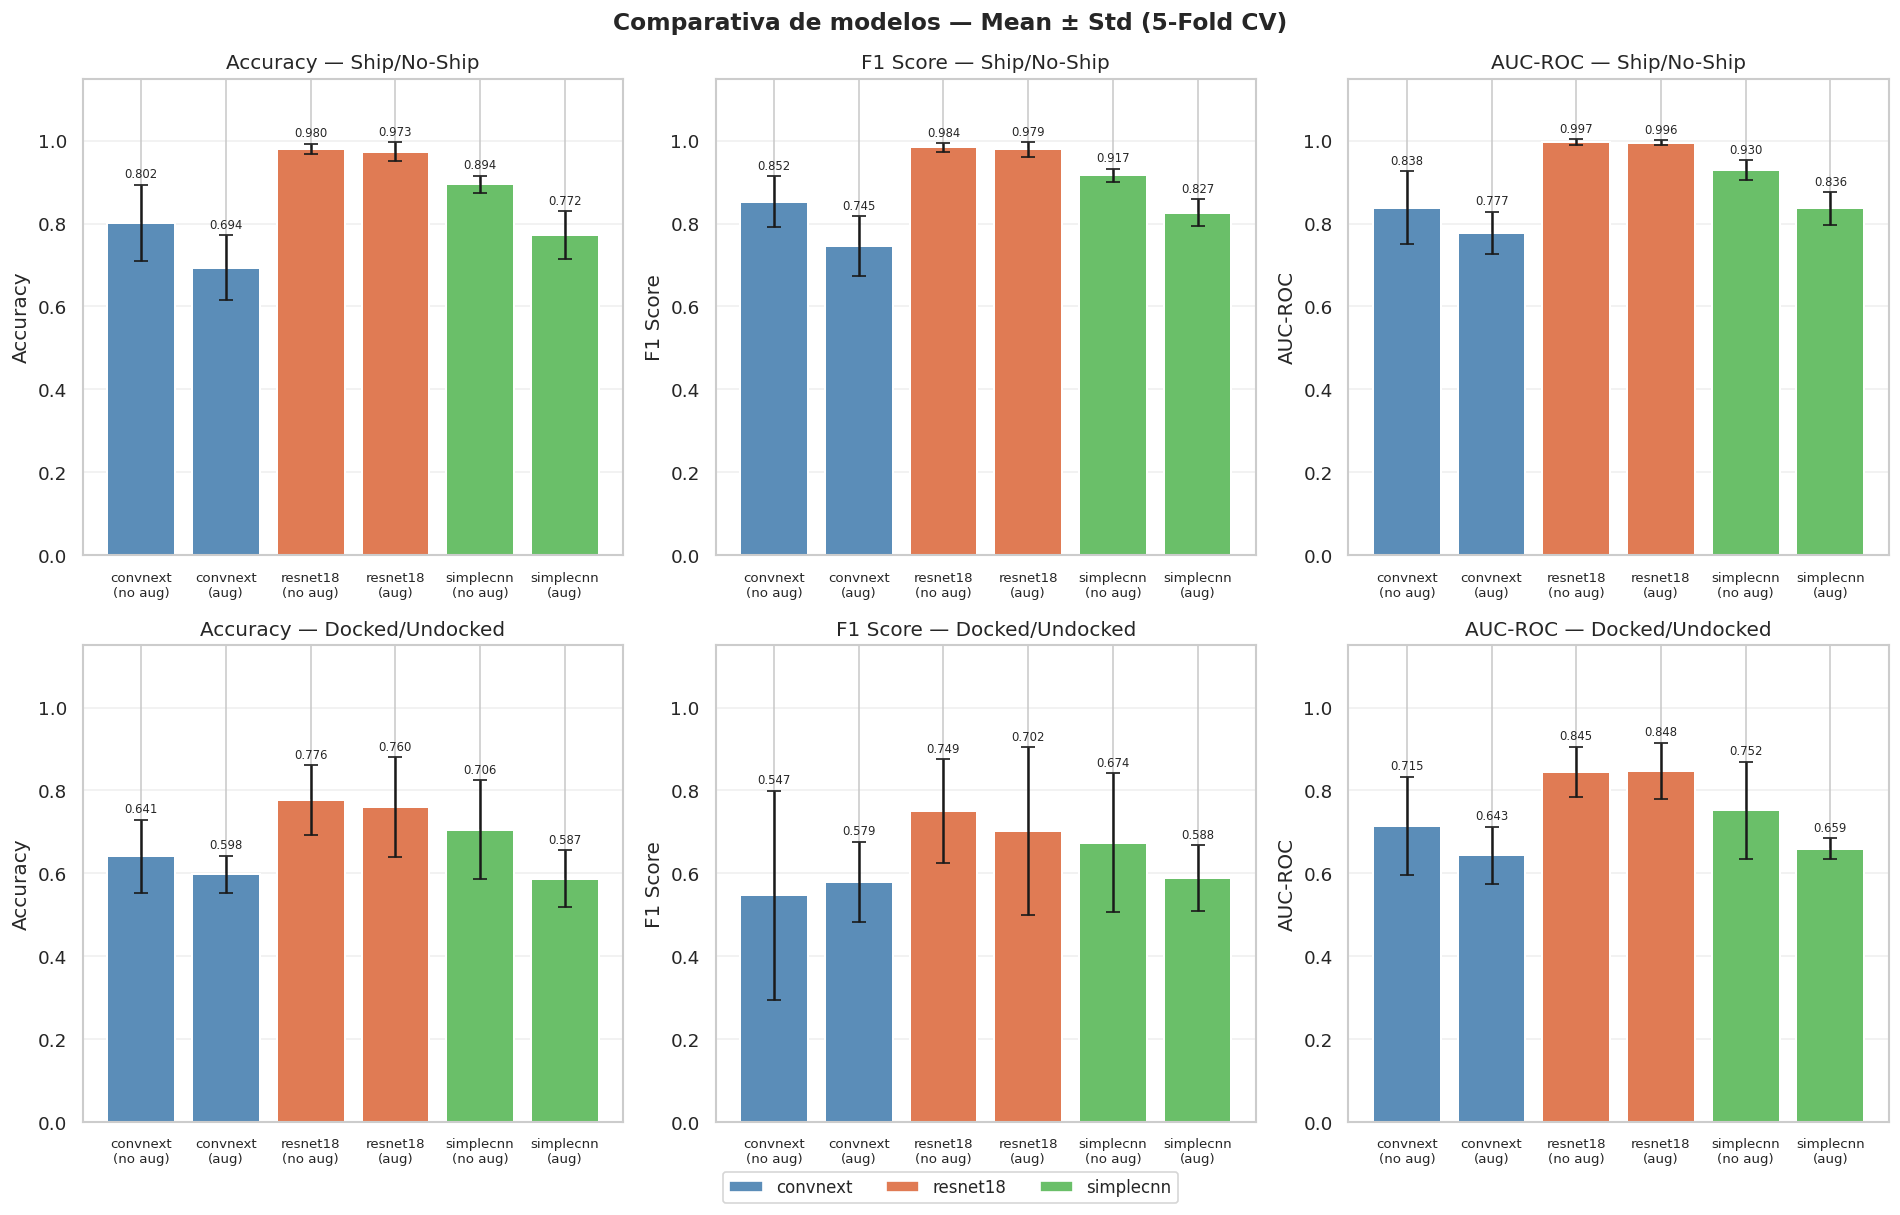
\includegraphics[width=0.92\textwidth]{comparison_all_models.png}
    \caption{Comparativa de todos los modelos para ambas tareas (Accuracy, F1 y
             AUC-ROC). Las barras de error representan la desviación típica
             entre folds.}
    \label{fig:comparison}
\end{figure}

\textsc{ResNet18} mantiene su ventaja con un AUC-ROC de 0.861, pero la brecha
con los modelos entrenados desde cero es menor que en Ship. La varianza entre
folds es mayor en todos los modelos, lo que refleja la mayor dificultad
intrínseca de la tarea y el tamaño más reducido del dataset (184 imágenes).

El \textit{data augmentation} empeora los resultados en esta tarea, especialmente
para \textsc{SimpleCNN}. Con tan pocas muestras, las transformaciones pueden
introducir variabilidad artificial que dificulta aprender las relaciones
espaciales clave para distinguir el estado de atraque.

\begin{figure}[H]
    \centering
    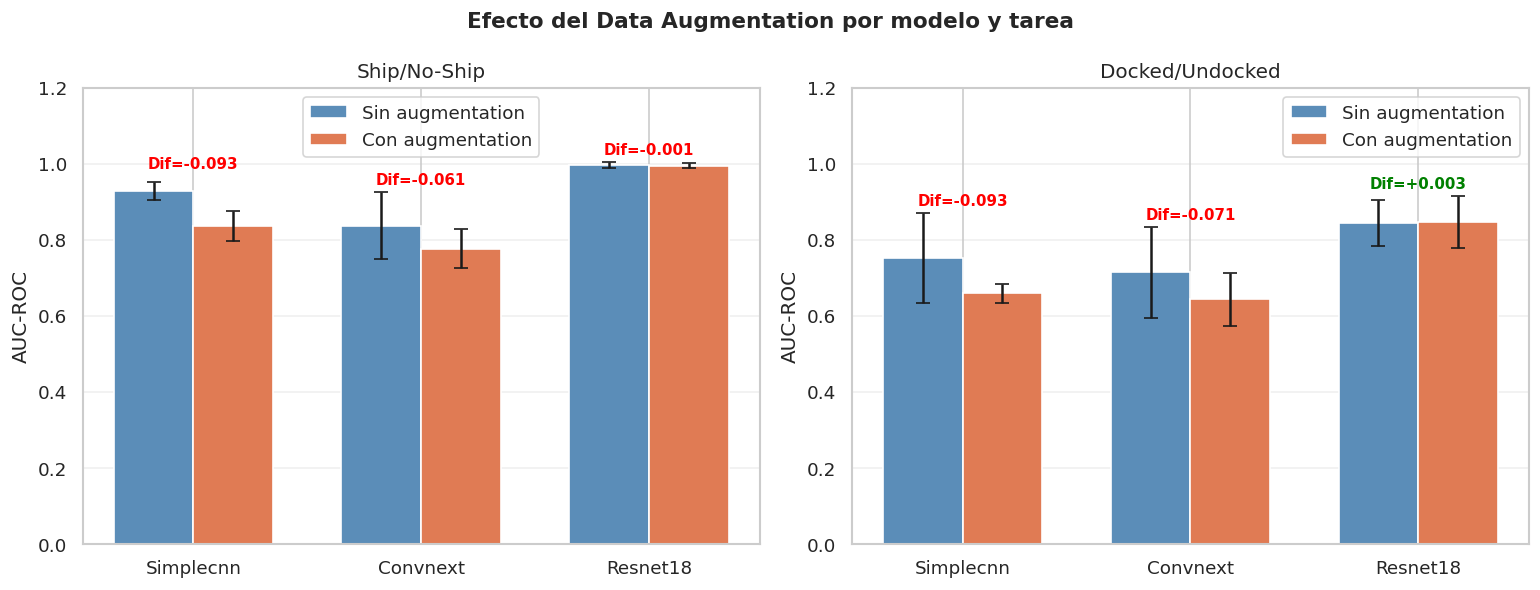
\includegraphics[width=0.72\textwidth]{augmentation_effect.png}
    \caption{Efecto del \textit{data augmentation} sobre el AUC-ROC en ambas tareas.
             En Ship el efecto es neutro; en Docked es sistemáticamente negativo.}
    \label{fig:augmentation}
\end{figure}

% ══════════════════════════════════════════════════════════════════════════════
\section{Experimento de Transfer Learning Inter-tarea}

\subsection{Motivación y diseño}

Dado el rendimiento moderado en la tarea Docked/Undocked, se plantea una
hipótesis: ¿puede el conocimiento adquirido durante el entrenamiento en
Ship/No-Ship mejorar el rendimiento en Docked/Undocked?

La intuición es que los modelos entrenados en Ship han aprendido a reconocer
la silueta y estructura visual de las embarcaciones - información que podría
ser directamente útil para determinar el estado de atraque. Esta estrategia
es especialmente relevante para \textsc{SimpleCNN}, que parte de pesos
aleatorios y se beneficiaría de una inicialización más informativa.

El procedimiento es el siguiente para cada fold $k$:
\begin{enumerate}
    \item Cargar el checkpoint del modelo entrenado en Ship (fold $k$).
    \item Reinicializar la capa de clasificación final con pesos Xavier.
    \item Descongelar todos los parámetros y fine-tunear sobre el conjunto
          Docked con $\text{lr} = 10^{-4}$.
\end{enumerate}

\subsection{Resultados y discusión}

\begin{table}[H]
\centering
\caption{Comparativa transfer learning vs.\ entrenamiento desde cero
         en la tarea Docked/Undocked (AUC-ROC, media $\pm$ desv. típica).}
\label{tab:transfer}
\small
\begin{tabular}{llC{2.2cm}C{2.2cm}C{2cm}}
\toprule
\textbf{Modelo} & \textbf{Aug} & \textbf{Desde cero} & \textbf{Transfer} & \textbf{$\Delta$} \\
\midrule
\multirow{2}{*}{SimpleCNN}  & No & 0.752 ± 0.117 & 0.736 ± 0.131 & $-$0.016 \\
                             & Sí & 0.660 ± 0.026 & 0.656 ± 0.103 & $-$0.004 \\
\midrule
\multirow{2}{*}{ResNet18}   & No & 0.861 ± 0.055 & 0.841 ± 0.067 & $-$0.020 \\
                             & Sí & 0.855 ± 0.068 & 0.860 ± 0.065 & $+$0.005 \\
\bottomrule
\end{tabular}
\end{table}

\begin{figure}[H]
    \centering
    \includegraphics[width=0.92\textwidth]{transfer_vs_baseline_docked.png}
    \caption{Comparativa visual entre entrenamiento desde cero y transfer
             learning (Ship $\to$ Docked) para tres métricas y dos configuraciones
             de augmentation. El delta sobre cada par indica la diferencia absoluta.}
    \label{fig:transfer}
\end{figure}

La hipótesis \textbf{no se confirma}: el transfer learning inter-tarea no
mejora los resultados base de forma consistente. Los deltas son pequeños y
mayoritariamente negativos.

Esto puede explicarse por dos motivos complementarios:

\begin{itemize}
    \item \textbf{Para ResNet18}: el modelo ya parte de ImageNet, que
          proporciona features visuales de muy alta calidad. El entrenamiento
          en Ship/No-Ship no añade información relevante que ImageNet no
          proporcionara ya.

    \item \textbf{Para SimpleCNN}: las features aprendidas para detectar la
          \textit{presencia} de un barco (bordes, silueta global) no son las
          mismas que las necesarias para determinar su \textit{posición relativa}
          respecto al muelle. La tarea Docked/Undocked exige razonar sobre la
          relación espacial entre el barco y la infraestructura portuaria, lo que
          requiere features de mayor nivel semántico que las aprendidas en Ship.
\end{itemize}

\end{document}
